\documentclass[../MasterThesis.tex]{subfiles}
\graphicspath{ {./assets/images/} }


%----------------------------------------------------------------------------
%----------------------------------------------------------------------------

\begin{document}
	
	

%---------------------------------------------------------------------------
\newpage
%---------------------------------------------------------------------------

\section{Technical Background} \label{section:technicalbackground}


In this Chapter, the structure and usage of the Melt framework is explained and an overview of video streaming components and addition components is given.


%---------------------------------
\subsection{Melt} \label{subsection:melt}
\subsubsection*{Structure of the Melt framework}

The Melt framework (MLT/Melt) is a multimedia framework as a command-line (CLI) tool that can be used for video editing and playback. It is written in C and provides a set of tools, libraries, and services for handling multimedia content, including video and audio.~\cite{melt} 


A variety of tasks can be performed with Melt, including the application of filters on audio or video files, and converting data between different formats. 

In the following, the structure of the Melt framework will be briefly explained. For this, the documentation as well as the code of the framework are taken into consideration.~\cite{melt, melt_code}

\textit{Producer}, \textit{Consumer} and \textit{MLT frame objects} are fundamental components in the Melt framework.

A \textit{MLT frame object} is a data structure that is used for representing multimedia content. 
It is a container that holds multimedia data. Each \textit{MLT frame object} contains a single uncompressed frame image and its associated audio samples. These frame objects can be processed individually, which allows the user to manipulate and transform multimedia content efficiently.
\textit{MLT frame objects} can store the multimedia data in various formats and they support metadata annotations, which allows to attach additional information or properties to the multimedia content. This includes filters, which are discussed in Section~\ref{subsection:meltfilter}.


A \textit{Producer} generates or provides data -- it produces the \textit{MLT Frame objects}. 
It reads data from files or other data sources. The \textit{Producer} serves as the starting point of the data processing pipeline in Melt. It retrieves the raw data and passes it on to other components, for example the \textit{Consumer}. This can be seen in Figure~\ref{fig:producer_consumer}.

A \textit{Consumer} requests \textit{MLT Frame objects} from the producer.
It is responsible for consuming or processing the data that was produced by the \textit{Producer} or other components that are between the \textit{Producer} and \textit{Consumer}. 
The \textit{Consumer} represents the endpoint of the data processing pipeline and produces the final output or results.



\begin{figure}[H]
	\centering
	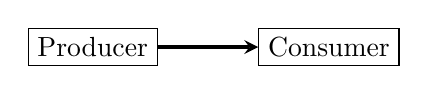
\begin{tikzpicture}
		% Nodes
		\node[draw, rectangle] (producer) at (0,0) {Producer};
		\node[draw, rectangle] (consumer) at (3,0) {Consumer};
		% Arrows
		\draw[->,>=stealth, line width=1.2pt] (producer) -- (consumer);
	\end{tikzpicture}
	\caption{Producer-Consumer Relationship}
	\label{fig:producer_consumer}
\end{figure}

Applying filters in the Melt framework is a technique for manipulating multimedia content, including videos. 
Melt filters can perform a wide range of operations, including colour correction, blurring, sharpening, cropping, resizing, and many others. A list of the filters can be found on the Melt website.~\cite{melt_filters}

To apply a filter in Melt, a filter instance has to be created and its parameters have to contain the name of the filter and, if needed, the filter parameters and values for those.

Filters are processing units that manipulate the multimedia data as it flows through the pipeline. They are placed between the producer and consumer, allowing them to modify the data before it reaches the consumer. This can be seen in Figure~\ref{fig:producer_filter_consumer}.



\begin{figure}[H]
	\centering
	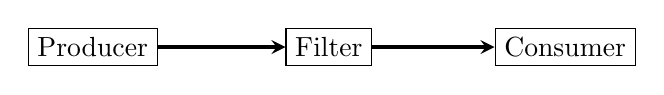
\begin{tikzpicture}
		% Nodes
		\node[draw, rectangle] (producer) at (0,0) {Producer};
		\node[draw, rectangle] (filter) at (3,0) {Filter};
		\node[draw, rectangle] (consumer) at (6,0) {Consumer};
		% Arrows
		\draw[->,>=stealth, line width=1.2pt] (producer) -- (filter);
		\draw[->,>=stealth, line width=1.2pt] (filter) -- (consumer);
	\end{tikzpicture}
	\caption{Producer-Filter-Consumer Relationship}
	\label{fig:producer_filter_consumer}
\end{figure}



\subsubsection*{Usage of the Melt framework}


In this Section, the usage of the Melt framework is explained with code examples and the explanation of those. This is based on the implemented code for this project, the code of the Melt framework and the Melt documentation.~\cite{melt}

The in the following described code structure refers to the creation of the necessary melt components to apply a filter.


\begin{description}[font=\normalfont\color{RedViolet!80!black}, style=nextline]
	
	%-----------------------------------------------
	\item[Initialise the factory] 
	
	This command initializes the Melt factory, to set up the environment for creating and managing multimedia objects.
	
	\begin{lstlisting}[language=C, numbers=none, basicstyle=\footnotesize\ttfamily, belowskip=0pt, aboveskip=9pt]
	mlt_factory_init(const char * directory); \end{lstlisting}

	The function takes a directory path as an optional parameter. In this directory, custom modules can bes stored, which can then override the default settings and the \texttt{MLT\_REPOSITORY} environment variable. 
	
	
	%-----------------------------------------------	
	\item[Create a profile]
	
	In this line, a multimedia profile is created to define the video properties.
	
	\begin{lstlisting}[language=C, numbers=none, basicstyle=\footnotesize\ttfamily, belowskip=0pt, aboveskip=9pt]
	mlt_profile profile = mlt_service_profile(mlt_service self); \end{lstlisting}
	
	The function \texttt{mlt\_service\_profile()} retrieves the profile that is associated with a given service. It takes a service as a parameter and returns its profile.
	
	


	%-----------------------------------------------	
	\item[Create a producer] 

	In this command, a producer object is created. The producer object generates or provides the data.

	\begin{lstlisting}[language=C, numbers=none, basicstyle=\footnotesize\ttfamily, belowskip=0pt, aboveskip=9pt]
	mlt_producer producer 
			= mlt_factory_producer(mlt_profile profile,
															const char* service,
															const void* resource); \end{lstlisting}
																						  
	The function \texttt{mlt\_factory\_producer()} creates a producer based on the profile, service and resources, which are the parameters of this function.


	
	
	%-----------------------------------------------	
	\item[Create properties] 
	
	This line retrieves the properties that are associated with a as parameter given producer in a property object.
	
	\begin{lstlisting}[language=C, numbers=none, basicstyle=\footnotesize\ttfamily, belowskip=0pt, aboveskip=9pt]
	mlt_properties properties 
			= MLT_PRODUCER_PROPERTIES(producer); \end{lstlisting}
	
	The macro \texttt{MLT\_PRODUCER\_SERVICE} internally accesses the properties of the producer.
	
	
	
	%-----------------------------------------------	
	\item[Create a consumer] 
	
	This line creates a consumer object, that processes the data.
	
	\begin{lstlisting}[language=C, numbers=none, basicstyle=\footnotesize\ttfamily, belowskip=0pt, aboveskip=9pt]
	mlt_consumer consumer 
			= mlt_factory_consumer(mlt_profile profile, 
															const char* service, 
															const void* input); \end{lstlisting}
																
	The function \texttt{mlt\_factory\_consumer()} creates a consumer object, basedon the as parameter provided profile, service and optional input. If the service object is not specified, it defaults to \texttt{MLT\_CONSUMER}.
											
																
	% TODO: seems to take properties as first parameter in codemill code? Is property and prfile the same?
	
	
	
	%-----------------------------------------------
	\item[Create a filter] 
	
	In this command, a filter is created. The name of the filter is given as an argument in form of a String.
	
	\begin{lstlisting}[language=C, numbers=none, basicstyle=\footnotesize\ttfamily, belowskip=0pt, aboveskip=9pt]
	mlt_filter filter = mlt_factory_filter(mlt_profile profile, 
																					const char* service, 
																					const void* input); \end{lstlisting}
														
	The \texttt{mlt\_factory\_filter()} function retrieves a filter based on the parameters. Those are the profile, the name of the filter as service and an optional argument of the filter.



	%-----------------------------------------------
	\item[Create and set filter properties] 

	This code creates a property object and sets the filter properties.

	\begin{lstlisting}[language=C, numbers=none, basicstyle=\footnotesize\ttfamily, belowskip=0pt, aboveskip=9pt]
	mlt_properties filter_properties 
			= mlt_filter_properties(filter); \end{lstlisting}

	The function \texttt{mlt\_filter\_properties()} retrieves the properties of a filter. The filter is given as a parameter.

	\begin{lstlisting}[language=C, numbers=none, basicstyle=\footnotesize\ttfamily, belowskip=0pt, aboveskip=9pt]
	mlt_properties_set(mlt_properties self,
											const char* name,
											const char* value); \end{lstlisting}

	The function \texttt{mlt\_properties\_set()} assigns a new value to a property, in this case to a filter. The parameters are the filter properties, that were retrieved in the previous step, and the filter parameters and associated values as strings.
	
	
	
	
	%-----------------------------------------------
	\item[Connect elements] 
	
	Connect the filter to the producer and consumer to filter, if a filter is applied.
	
	\begin{lstlisting}[language=C, numbers=none, basicstyle=\footnotesize\ttfamily, belowskip=0pt, aboveskip=9pt]
	mlt_filter_connect( mlt_filter self, 
											mlt_service producer , 
											int index ); \end{lstlisting}

	The function \texttt{mlt\_filter\_connect} takes the filter and the producer as parameters and connects them.
	
	\begin{lstlisting}[language=C, numbers=none, basicstyle=\footnotesize\ttfamily, belowskip=0pt, aboveskip=9pt]
	mlt_consumer_connect( mlt_consumer self, 
												mlt_service producer ); \end{lstlisting}

	The function \texttt{mlt\_filter\_connect} takes the consumer and the filter as parameters and connects them.
	
	
	If no filter is applied, the producer is being connected to the consumer directly.
	
	\begin{lstlisting}[language=C, numbers=none, basicstyle=\footnotesize\ttfamily, belowskip=0pt, aboveskip=9pt]
	mlt_consumer_connect(mlt_consumer self, 
												mlt_service producer); \end{lstlisting}
	
	The function \texttt{mlt\_filter\_connect} takes the consumer and the producer as parameters and connects them.
	
	
	%-----------------------------------------------
	\item[Start consumer] 
	
	This line starts the consumer.
	
	\begin{lstlisting}[language=C, numbers=none, basicstyle=\footnotesize\ttfamily, belowskip=0pt, aboveskip=9pt]
	mlt_consumer_start(mlt_consumer self);	\end{lstlisting}

	The function \texttt{mlt\_consumer\_start()} initiates the consumer in the Melt framework. It takes the consumer object as a parameter. 
	
	
	
	
	
	%-----------------------------------------------
	\item[Close the components]
	
	The following functions are responsible for closing the associated component within the Melt framework. These functions mark the end of a Melt process by closing and cleaning up resources.
	
	\begin{lstlisting}[language=C, numbers=none, basicstyle=\footnotesize\ttfamily, belowskip=0pt, aboveskip=9pt]
	mlt_consumer_close(mlt_consumer self); 
	mlt_producer_close(mlt_producer self); 
	mlt_profile_close(mlt_profile profile); 
	mlt_factory_close();
	\end{lstlisting}
	
	
\end{description}










%-------------------------------------------------------------------------------------------------------
%-------------------------------------------------------------------------------------------------------
\subsection{Overview of Video Streaming Components}
\label{subsection_OverviewVideoStreamingComponents}

In this Section, an overview over video streaming components, that are relevant for this thesis project, is given.

Transcoding is the conversion of one digital data format into another.~\cite{transcoding}

One form of video transcoding is the compression of videos with h.264.
The video compression standard h.264 can be used to compress and decompress video streams in the context of real-time communication.~\cite{transcoding, h264}
	

File formats like Audio Video Interleave (AVI) often serve as input files for video transcoding processes.
AVI can contain audio and video information to allow synchronized playback of audio and video components. 
It is a container format, which means that it can contain multiple streams of audio and video data, along with other multimedia data such as subtitles.~\cite{avi}


AVI files can undergo transcoding to optimize their compression, compatibility, or quality, with h.264 being a commonly used codec for such purposes.~\cite{h264}


Web Real-Time Communication (WebRTC), is a free, open-source project for real-time communication between web browsers and other applications, that was developed by Google in 2011. It enables direct peer-to-peer (P2P) communication without the need for intermediary servers.~\cite{webrtc}
	

WebRTC supports various video codecs, including h.264, which is used for video conferencing, streaming, and other real-time applications. The video streams exchanged between the browser and the backend are encoded and decoded using h.264.~\cite{h264}





%-------------------------------------------------------------------------------------------------------
%\subsubsection*{Named Pipe} 

%A named pipe is a type of interprocess communication (IPC) mechanism. It provides a way for processes to pass data to each other and it is bidirectional. 
%Named pipes follow a First-In-First-Out (FIFO) structure: The first data written into the pipe is the first data to be read. This maintains a sequential order for data transmission.
%A traditional pipe is \textit{unnamed} and terminates when its process terminates. A named pipe can last beyond the life of the process, as long as the system is running.~\cite{namedpipe}





%-------------------------------------------------------------------------------------------------------
%\subsubsection*{REST} 


Representational State Transfer (REST) is an architecture for network applications. A REST Application Programming Interface (API) exposes a set of endpoints (URLs) that allow communication between different software systems over the internet with hypertext transfer protocol (HTTP) methods.~\cite{IEEE_Rest, webservice, Nodejs_Rest}



	
Just-In-Time (JIT), in the context of video streaming, refers to a dynamic software solution employed for real-time video transformation. It is used for on-the-fly conversion of video files, optimizing them for streaming. The process includes the transformation of a video file, potentially one with non-web-friendly formats, into a more suitable format for the playback in web browsers.~\cite{JIT_IEEE}



%-------------------------------------------------------------------------------------------------------
\subsection{Overview of Additional Components}
\label{subsection:overview_additional_components}


This Section introduces additional components that are relevant for the system's functionality.


Docker provides an isolated environment where applications can run. It's a platform that enables the usage of these isolated environments, that are called Docker containers.~\cite{docker}


Node.js enables the execution of JavaScript code outside of a web browser.
Its enables developers to use JavaScript both on the client and server sides of web applications. 
Node.js has an open-source community that contributes to its evolution. This community-driven development model has led to a big selection of modules and libraries.~\cite{nodejs, RM_Frontend, ap3_docs}


To manage project dependencies and packages for Node.js, tools like Yarn or npm (Node Package Manager) can be used. These package managers allow developers to install, update, and manage libraries and tools used in the project, by providing a centralized repository of libraries and tools.~\cite{RM_Frontend, npmyarn}



Web services are software systems for communication between different applications over a network. 
They allow data exchange and function calling across platforms and programming languages. 
Java-based web services are commonly used in modern software development, due to the robustness and scalability of the Java platform for building distributed systems over the web.
Web services enable machine-to-machine (M2M) interaction. This is the communication and data exchange between devices or systems.~\cite{webservice}



%-------------------------------------------------------------------------------------------------------
\subsection{Protocol Buffer}
\label{subsection:protocolbuffer}


Protocol buffers are developed by Google. They compress data for sending it faster over a network. The protocol buffer provides an efficient binary data format. The structure of this format is defined in a \texttt{.proto} file. Those files are used to generate code for reading and writing to the protocol buffer. Because of the compression, it is useful for sending data in networks.~\cite{protobuffer}

In this project, Protocol Buffers version 2 (proto2) was used. In the first line of the \texttt{.proto} file, the syntax is defined with the proto version that is being used. This can be seen for proto2 in the following:

\begin{lstlisting}[style=protobufStyle, numbers=none]
	syntax = "proto2";
\end{lstlisting}

\begin{description}[font=\normalfont\color{RedViolet!80!black}, style=nextline]
	

%---------------------------------------------------------------------------------------------------------
\item[Messages and Fields] 

Data structures are defined using message declarations. Messages can contain fields for the data, each with a unique identifier and a specified data type. The data types for proto2 can be seen in Table~\ref{table:proto2_data_types}.~\cite{proto2_doc}


\begin{table}[H]
	\centering

	\begin{tabular}{ll}
		\toprule
		\textbf{Data Type} & \textbf{Description} \\
		\midrule
		double & Double-precision floating-point number \\
		float & Single-precision floating-point number \\
		int32 & Signed 32-bit integer \\
		int64 & Signed 64-bit integer \\
		uint32 & Unsigned 32-bit integer \\
		uint64 & Unsigned 64-bit integer \\
		sint32 & Signed 32-bit integer (suitable for negative numbers) \\
		sint64 & Signed 64-bit integer (suitable for negative numbers) \\
		fixed32 & Unsigned 32-bit integer (four bytes) \\
		fixed64 & Unsigned 64-bit integer (eight bytes) \\
		sfixed32 & Signed 32-bit integer (four bytes) \\
		sfixed64 & Signed 64-bit integer (eight bytes) \\
		bool & Boolean value (true or false) \\
		string & Variable-length text string  \\
		bytes & Variable-length sequence of bytes \\
		\bottomrule
	\end{tabular}
	\caption{Data types for fields in Protocol Buffers (proto2).~\cite{proto2_doc}}
	\label{table:proto2_data_types}
\end{table}

In the following, an example message is shown and described.
The example message represents a person's information, including their name, age, and email address. This is defined as follows:

\begin{lstlisting}[style=protobufStyle, numbers=none]
	message Person {
		required string name = 1;
		required int32 age = 2;
		optional string email = 3;
	}
\end{lstlisting}

Person is the name of the message and name, age, and email are the fields of the message with the data types \texttt{string} and \texttt{int32}.
The keywords \texttt{required} and \texttt{optional} define whether the field is mandatory or optional.
The numbers $1$, $2$ and $3$ are the fields unique identifiers.


%---------------------------------------------------------------------------------------------------------
\item[Enums] 

Proto2 supports the definition of enumeration types as enum.
Enums allow for the declaration of a set of named constants, each associated with a unique integer value.
This can be used for representing a fixed set of options or states within a message definition.~\cite{protobuffer, proto2_doc}

In the following, an example enum is shown and described. 
It represents the gender of a person and is defined as follows:

\begin{lstlisting}[style=protobufStyle, numbers=none]
	enum Gender {
		UNKNOWN = 0;
		MALE = 1;
		FEMALE = 2;
		DIVERSE = 3;
	}
\end{lstlisting}

Gender is the name of the enum and UNKNOWN, MALE, and FEMALE are the enum constants with the associated integer values $1$, $2$ and $3$.
It allows to represent the gender options unknown, male, or female, providing a way to represent a fixed set of options or states.



\end{description}


	
\end{document}